\documentclass[final]{beamer}

\usepackage[T1]{fontenc}
 \usepackage[utf8]{luainputenc}
\usepackage{lmodern}
\usepackage[size=custom, width=122,height=91, scale=1.2]{beamerposter}
\usetheme{gemini}
\usecolortheme{bgu}
\usepackage{graphicx}
\usepackage{booktabs}
\usepackage{tikz}
\usepackage{pgfplots}
\usepgfplotslibrary{statistics}
\pgfplotsset{compat=1.14}
%\usepackage{anyfontsize}


\newlength{\sepwidth}
\newlength{\colwidth}
\setlength{\sepwidth}{0.025\paperwidth}
\setlength{\colwidth}{0.3\paperwidth}

\newcommand{\separatorcolumn}{\begin{column}{\sepwidth}\end{column}}



\title{Rubik's Mathematics: A Twist on Numbers}

\author{Jeremy Huang and Benedict Antonious}

\institute[shortinst]{University of Colorado Boulder}



\logoleft{
\includegraphics[height=4.5cm]{logos/BoulderLogo.png}}


\begin{document}

\begin{frame}[t]
\begin{columns}[t]
\separatorcolumn

\begin{column}{\colwidth}

  \begin{block}{Abstract}
    \large The Rubik's Cube, an iconic 3D puzzle, has captured the imagination of enthusiasts and mathematicians alike for decades. This poster delves into the mathematical intricacies of the Rubik's Cube. We investigate the cube's symmetry, its staggering number of possible permutations, and the use of computer aided proof-assistants to calculate the algorithms to solve the Rubik's Cube. Whether you're a puzzle enthusiast or a math fanatic, this poster invites you to embark on a fascinating journey into the world of Rubik's Cube mathematics.


  \end{block}

  \begin{block}{Combinations of a Rubik's Cube}

    \large There are three (four if you count the not-visible core) types of pieces:

    \begin{itemize} %Talk about centers/edges/corners
      \item \textbf{Corners:} 8 of these on each corner of the cube
      \item \textbf{Edges:} 12 of these connecting adjacent corners
      \item \textbf{Centers:} 6 of these on each face of the cube
    \end{itemize}

    There are $8!$ ways we can permute the corner pieces to the corners of a cube, and $12!$ ways 
    we can permute the edge pieces into the 12 edge slots of a cube. There are $3^8$ ways we can orient 
    the corner pieces and $2^{12}$ ways we can the edge pieces. We also have to divide by $12$, 
    since some states are impossible. This yields the final formula: \\

    $$ \displaystyle\frac{8!\cdot 12! \cdot 3^8 \cdot 2^{12}}{12} = 43252003274489856000 $$ \\

    \begin{figure}
      \centering
                    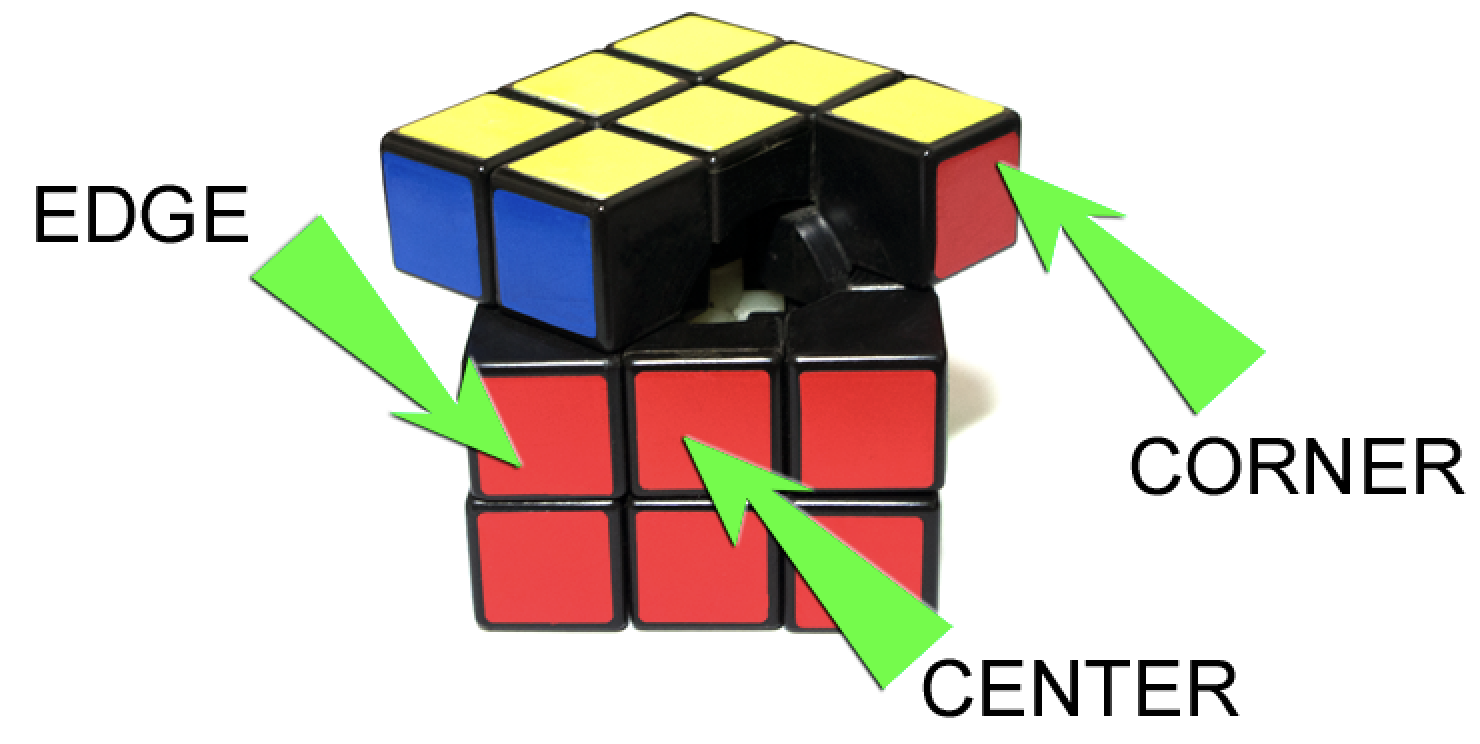
\includegraphics[width=0.6\textwidth]{logos/rubikspieces.png}
    \end{figure}

  \end{block}

  \begin{block}{How big is 43 Quintillion?}

    \large 
    %Imagine we find a new, unique Rubik's cube combination every second. There are
    %about 31 million seconds in a year, so it would take more than 1.3 trillion years. \\
    %Imagine we started doing this during the Dinosaur Age: we would only get to 2 quadrillion combinations. \\
    %We would have to repeat the process more than 20,000 times to reach all 43 quintillion combinations! \\
    Imagine we had a dollar for each rubik's cube combination there was. If were to lay one layer of one dollar bills in
    Colorado, it would take 25 trillion dollars. We would have to stack that another 2 million times to use all of our money. \\
    The stack would be about the same height of the tallest building in Denver. In other words,
    the money would cover all of Colorado in a layer as tall as a skyscraper.
    \begin{figure}
      \centering
                    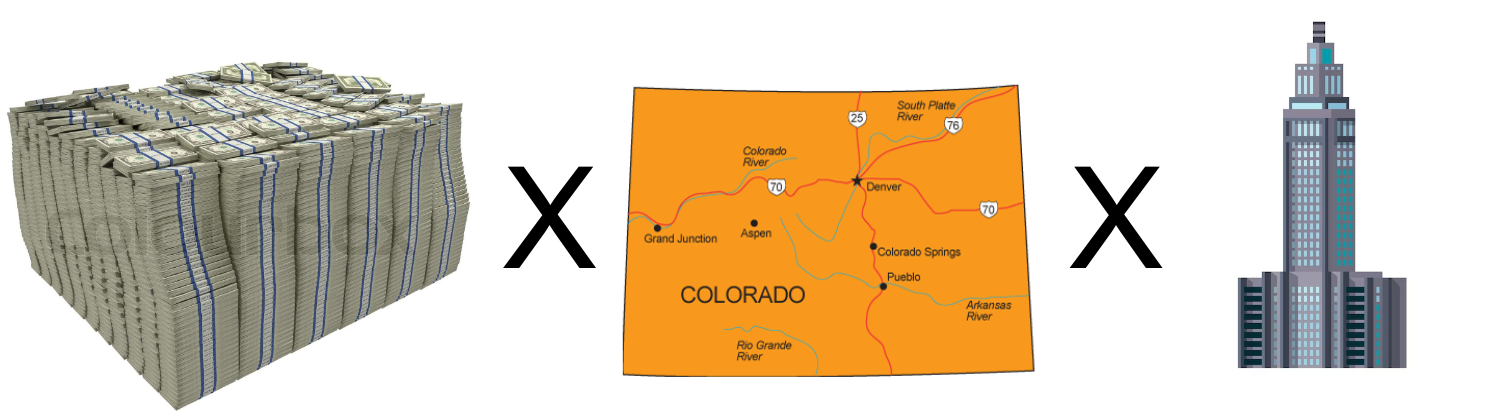
\includegraphics[width=0.9\textwidth]{logos/moneyvisual.png}
    \end{figure}

  \end{block}

\end{column}

\separatorcolumn

\begin{column}{\colwidth}

  \begin{block}{Solving a Rubik's Cube}

<<<<<<< Updated upstream
    \large A popular method for speed-solving is CFOP(used by many world record holders) where you create a Center \textbf{Cross}, solve the First two layers(\textbf{F2L}), Orient the last layer(\textbf{OLL}), and Permute the last layer(\textbf{PLL}). 
    We can figure out the maximum number of moves it would take for a solve using CFOP by going adding up the maximum steps of each step: 
=======
    \large CFOP solving method: 
    \begin{figure}
      \centering
      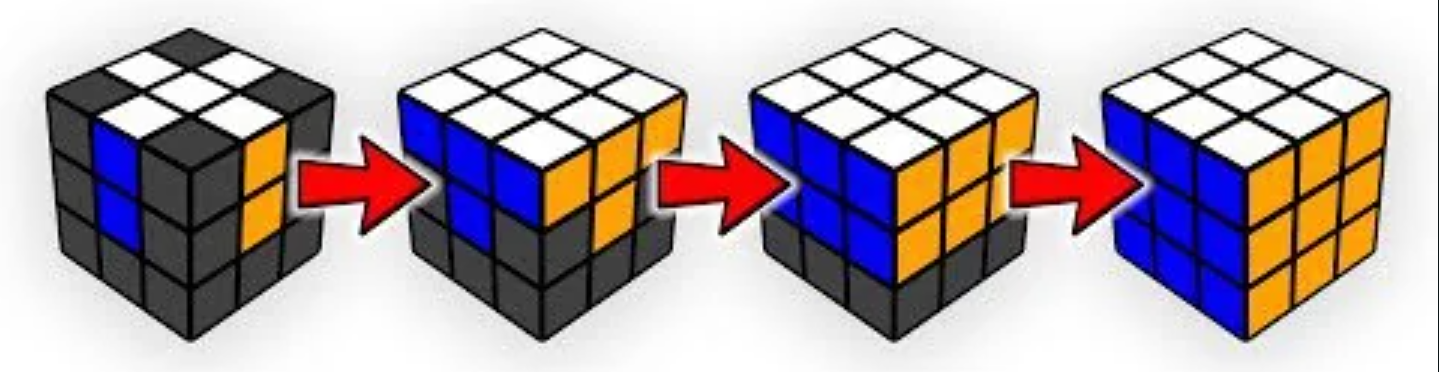
\includegraphics[scale = 2]{logos/CFOP.PNG}
    \end{figure}
>>>>>>> Stashed changes
    \begin{enumerate}
      \item[C] Center Cross - 8 moves max
      \item[F] First 2 Layers(F2L) - 24-28 moves max
      \item[O] Orientation of Last Layer(OLL) - 11 moves max
      \item[P] Permutation of Last Layer(PLL) - 14 moves max
    \end{enumerate}
<<<<<<< Updated upstream
    Across the four steps in CFOP we have a maximum of around 61 moves needed to solve a 3x3 Cube.

=======
    Across the four steps in CFOP we have about 60 moves needed to solve a 3x3 Cube.
    
    \begin{tikzpicture}
      \begin{axis} [
        height=12.0cm, width=25.0cm,
        xmin=0, xmax=50, xtick={0,5,10,15,...,50},
        ytick={1,2,3,4},
        yticklabels={P,O,F,C},
        legend style={at={(0.5,-0.2)}, anchor=north, legend columns=-1},
        ymin=0,ymax=5,
        /pgfplots/boxplot/box extend=0.3
    ]
        \addplot+ [
        boxplot prepared={
          median=15,
          upper quartile=16,
          lower quartile=13,
          upper whisker=24,
          lower whisker=2,
        },
        ] coordinates {};
        \addplot+ [
        boxplot prepared={
          median=10,
          upper quartile=12,
          lower quartile=8,
          upper whisker=18,
          lower whisker=4,
        },
        ] coordinates {};
        \addplot+ [
        boxplot prepared={
          median=30,
          upper quartile=33,
          lower quartile=25,
          upper whisker=48,
          lower whisker=4,
        },
        ] coordinates {};
        \addplot+ [
        boxplot prepared={
          median=6,
          upper quartile=8,
          lower quartile=5,
          upper whisker=13,
          lower whisker=1,
        },
        ] coordinates {};
      \end{axis}
    \end{tikzpicture}
>>>>>>> Stashed changes

  \end{block}

  \begin{block}{God's Algorithm and Number}

    \large God's Algorithm is a term used to refer to the optimal algorithm used to solve a cube in the least moves possible 
    while God's Number refers to the the number of moves in the worst case of God's Algorithm.
    In 2010, God's Number was proven to be 20. 
    
    
    
    Et rutrum ex euismod vel. Pellentesque ultricies, velit in fermentum
    vestibulum, lectus nisi pretium nibh, sit amet aliquam lectus augue vel
    velit. Suspendisse rhoncus massa porttitor augue feugiat molestie. Sed
    molestie ut orci nec malesuada. Sed ultricies feugiat est fringilla
    posuere. \\
    \begin{center}
    \begin{tikzpicture}[scale=1.13]
      \begin{axis}[xtick = {12,13,14,15,16,17,18,19,20},
          ymin=0, ymax=100, xmin = 12, xmax = 21, xlabel = \# of moves,
          area style, width=25cm,height=9cm, xticklabel style = {xshift=1.3cm}
          ]
        \tikzstyle{every node}=[font=\small]
      \addplot+[ybar interval,mark=no] plot coordinates { (0, 0) (1, 0) (2, 0) (3, 0) (4,0) (5,0) (6,0)
       (7,0) (8,0) (9,0) (10,0) (11,0) (12,0) (13,0) (14,0) (15, 0.2) (16, 2.5) (17, 27.7) (18, 67) (19, 3.5) (20,0) (21,0) };
        \node[] at (axis cs: 16.5,10) {2.5\%};
        \node[] at (axis cs: 17.5,36) {27.7\%};
        \node[] at (axis cs: 18.5,76) {67\%};
        \node[] at (axis cs: 19.5,12) {3.5\%};
        \node[] at (axis cs: 20.5, 10) {<0.1\%};
        \node[] at (axis cs: 14, 9) {<0.1\%};

      \end{axis}
      \end{tikzpicture}
    \end{center}

  \end{block}

  \begin{block}{Proof Assistants/Computer Aided proof}

    \large Nulla eget sem quam. Ut aliquam volutpat nisi vestibulum convallis. Nunc a
    lectus et eros facilisis hendrerit eu non urna. Interdum et malesuada fames
    ac ante \textit{ipsum primis} in faucibus. Etiam sit amet velit eget sem
    euismod tristique. Praesent enim erat, porta vel mattis sed, pharetra sed
    ipsum. Morbi commodo condimentum massa, \textit{tempus venenatis} massa
    hendrerit quis. Maecenas sed porta est. Praesent mollis interdum lectus,
    sit amet sollicitudin risus tincidunt non.

  \end{block}

\end{column}

\separatorcolumn

\begin{column}{\colwidth}

  \begin{block}{Applications to Speed Cubing}

    \large There are many different methods for Speed Cubing, all aimed at Solving
    the cube as fast as possible. This involves coming up with ways to use
    less moves and using easily executed algorithms. Here are a couple:

    \begin{table}
      \centering
      \begin{tabular}{l r r c}
        \toprule
        \textbf{Method} & \textbf{\# Turns} & \textbf{\# Algorithms} & \textbf{Average Times (s)} \\
        \midrule
        Beginner & 80-100 & 15 & 30-120 \\
        CFOP & 55-60 & 78 & 5-30 \\
        Roux & 45-50 & 100+ & 5-20 \\
        ZZ & 45-55 & 493 & 5-15 \\
        \bottomrule
      \end{tabular}
    \end{table}


  As more methods and algorithms get developed with the aid of computers,
  speed-cube times have been getting lower considerably:

  \begin{figure}
    \centering
      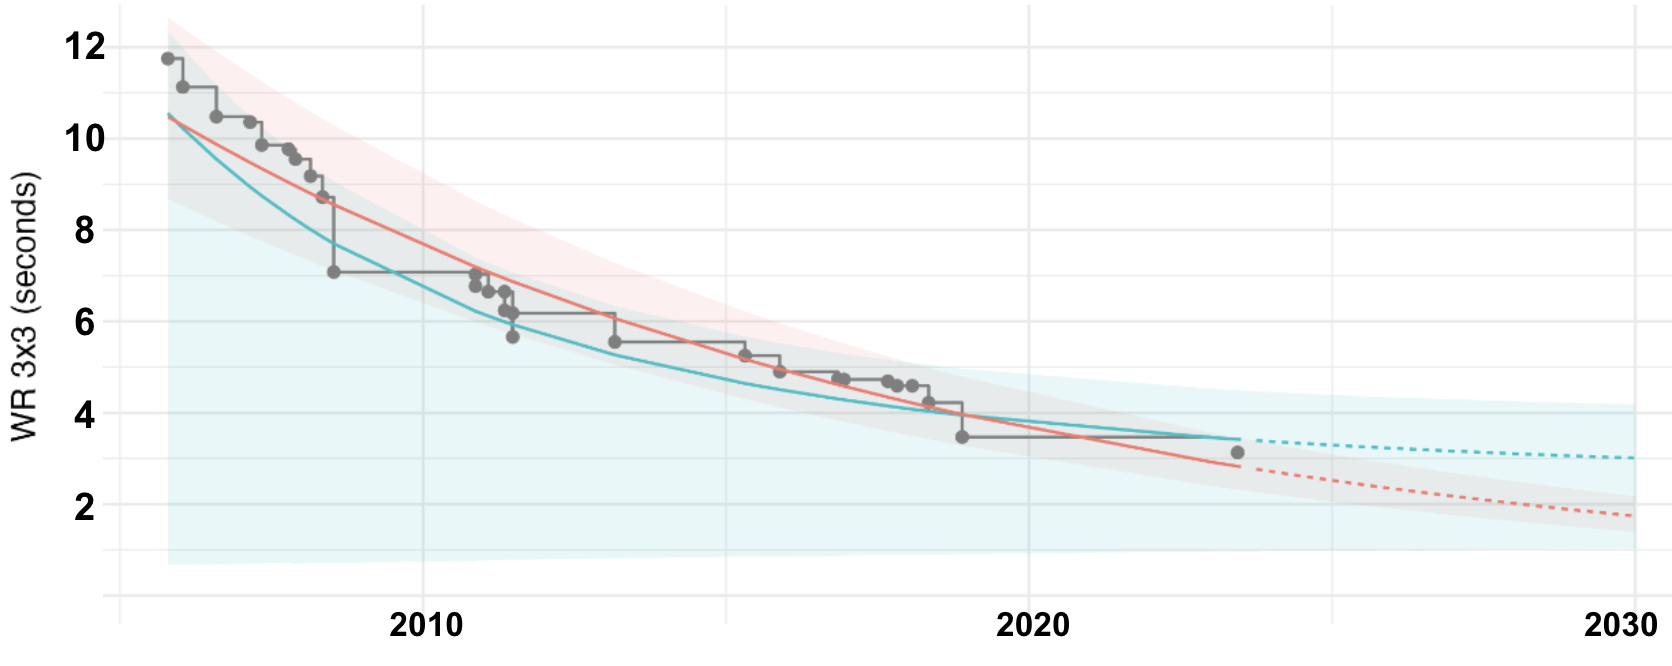
\includegraphics[width=1.0\textwidth]{logos/solveprogression.png}
  \end{figure}

  \end{block}

  \begin{block}{What about larger Rubik's Cubes?}
    
    \large Unsurprisingly, the number of possible combinations of larger Rubik's Cube scale exponentially \\
    
    \begin{itemize}
      \item \textbf{4x4:} 7.4 quattuordecillion ($7.5\cdot 10^{45}$) - 20s solve time
      \item \textbf{5x5:} 283 trevigintillion ($283 \cdot 10^{72}$) - 38s solve time
      \item \textbf{6x6:} Big number with 117 digits - 75s solve time
      \item \textbf{7x7:} Big number with 165 digits - 110s solve time
    \end{itemize}

    The general formula for the combinations on an $n \times n$ cube is: \\

    $$ \displaystyle 7! \cdot  3^6 \left( 24 \cdot 2^{10} \cdot 12!  \right)^{n \text{ mod} 2}
    (24!)^{\lfloor \frac{n-2}{2} \rfloor} \left( \displaystyle\frac{24!}{4!^{6}} 
    \right)^{\lfloor \left( \frac{n-2}{2} \right)^2 \rfloor} $$ \\


  \end{block}

  \begin{block}{References}

    \nocite{*}
    \footnotesize{\bibliographystyle{plain}\bibliography{poster}}

  \end{block}

\end{column}

\separatorcolumn
\end{columns}
\end{frame}

\end{document}
